

\documentclass[man,floatsintext]{apa6}
\usepackage{lmodern}
\usepackage{amssymb,amsmath}
\usepackage{ifxetex,ifluatex}
\usepackage{fixltx2e} % provides \textsubscript
\ifnum 0\ifxetex 1\fi\ifluatex 1\fi=0 % if pdftex
  \usepackage[T1]{fontenc}
  \usepackage[utf8]{inputenc}
\else % if luatex or xelatex
  \ifxetex
    \usepackage{mathspec}
  \else
    \usepackage{fontspec}
  \fi
  \defaultfontfeatures{Ligatures=TeX,Scale=MatchLowercase}
\fi
% use upquote if available, for straight quotes in verbatim environments
\IfFileExists{upquote.sty}{\usepackage{upquote}}{}
% use microtype if available
\IfFileExists{microtype.sty}{%
\usepackage{microtype}
\UseMicrotypeSet[protrusion]{basicmath} % disable protrusion for tt fonts
}{}
\usepackage{hyperref}
\hypersetup{unicode=true,
            pdftitle={Assessing sampling methods for generalization from RCTs: Modeling recruitment and participation},
            pdfauthor={Gleb Furman~\& James E. Pustejovsky},
            pdfborder={0 0 0},
            breaklinks=true}
\urlstyle{same}  % don't use monospace font for urls
\usepackage{graphicx,grffile}
\makeatletter
\def\maxwidth{\ifdim\Gin@nat@width>\linewidth\linewidth\else\Gin@nat@width\fi}
\def\maxheight{\ifdim\Gin@nat@height>\textheight\textheight\else\Gin@nat@height\fi}
\makeatother
% Scale images if necessary, so that they will not overflow the page
% margins by default, and it is still possible to overwrite the defaults
% using explicit options in \includegraphics[width, height, ...]{}
\setkeys{Gin}{width=\maxwidth,height=\maxheight,keepaspectratio}
\IfFileExists{parskip.sty}{%
\usepackage{parskip}
}{% else
\setlength{\parindent}{0pt}
\setlength{\parskip}{6pt plus 2pt minus 1pt}
}
\setlength{\emergencystretch}{3em}  % prevent overfull lines
\providecommand{\tightlist}{%
  \setlength{\itemsep}{0pt}\setlength{\parskip}{0pt}}
\setcounter{secnumdepth}{0}
% Redefines (sub)paragraphs to behave more like sections
\ifx\paragraph\undefined\else
\let\oldparagraph\paragraph
\renewcommand{\paragraph}[1]{\oldparagraph{#1}\mbox{}}
\fi
\ifx\subparagraph\undefined\else
\let\oldsubparagraph\subparagraph
\renewcommand{\subparagraph}[1]{\oldsubparagraph{#1}\mbox{}}
\fi

%%% Use protect on footnotes to avoid problems with footnotes in titles
\let\rmarkdownfootnote\footnote%
\def\footnote{\protect\rmarkdownfootnote}


  \title{Assessing sampling methods for generalization from RCTs: Modeling recruitment and participation}
    \author{Gleb Furman\textsuperscript{1}~\& James E. Pustejovsky\textsuperscript{1}}
    \date{}
  
\shorttitle{Assessing sampling methods for generalization from RCTs}
\affiliation{
\vspace{0.5cm}
\textsuperscript{1} University of Texas at Austin}
\usepackage{csquotes}
\usepackage{upgreek}
\captionsetup{font=singlespacing,justification=justified}

\usepackage{longtable}
\usepackage{lscape}
\usepackage{multirow}
\usepackage{tabularx}
\usepackage[flushleft]{threeparttable}
\usepackage{threeparttablex}

\newenvironment{lltable}{\begin{landscape}\begin{center}\begin{ThreePartTable}}{\end{ThreePartTable}\end{center}\end{landscape}}

\makeatletter
\newcommand\LastLTentrywidth{1em}
\newlength\longtablewidth
\setlength{\longtablewidth}{1in}
\newcommand{\getlongtablewidth}{\begingroup \ifcsname LT@\roman{LT@tables}\endcsname \global\longtablewidth=0pt \renewcommand{\LT@entry}[2]{\global\advance\longtablewidth by ##2\relax\gdef\LastLTentrywidth{##2}}\@nameuse{LT@\roman{LT@tables}} \fi \endgroup}

\begin{document}
\maketitle

Recently, randomized controlled trials (RCTs) have come under scrutiny for their limited generalizability due to inadequate sampling strategies (Stuart, Cole, Bradshaw, \& Leaf, 2011). RCTs provide a high level of internal validity as they demonstrate the causality of the impact being estimated. In education research, multisite RCTs, or multisite randomized trials (MRTs), are used to inform policy decisions by evaluating intervention impacts on a larger scale. Recruitment and randomization occurs at the organizational level (e.g.~schools), ostensibly increasing the diversity of settings in which the study takes place. In practice, however, the generalizability of MRTs is greatly limited by the sampling method being implemented. This is a major drawback for policymakers who are interested in generalizing treatment effects beyond the sample.

RCTs are commonly used in impact evaluations across many fields. Randomized treatment assignment ensures that estimated effects are causal, thus affording a higher level of internal validity. However, these effect estimates may be sample specific. If treatment effects are heterogeneous, then the impact of an intervention cannot be extrapolated beyond the study sample. This is a limiting feature of RCTs since policymakers seeking to implement interventions will have no way of gaguing effectivenes in their populaton of interest.

MRTs attempt to remedy this by studying the intervention on a larger scale. In educational research, for instance, multiple schools may be recruited to participate in a study, with each school randomly assigned to receive the intervention or continue buisiness as usual (BAU). This design offers greater external validity relative to the single-site variant because it enables the study of site-by-treatment interaction and formal tests of generalizability (Raudenbush \& Liu, 2000). Treatment effect estimates are said to be generalizable to schools that are \enquote{similar} to those in the study, however, the similarity can be difficult to define. Furthermore, if the sample of sites is too small or homogeneous, the scope of the generalization is greatly diminished.

Random sampling overcomes this limitation by selecting sites from a well-defined population with some known probability. When used in conjunction with randomized treatment assignment, this is known as dual randomization. Assuming no refusals during recruitment, and full compliance without attrition after assignment, this design enables unbiased estimation of the sample average treatment effect (SATE). Using the known sampling probabilities, the SATE can then be used to estimate the population average treatment effect (PATE).

In absence of random sampling, PATE can still be estimated by using propensity score techniques, provided there is sufficent overlap between the sample and the population (O'Muircheartaigh \& Hedges, 2014; Tipton, 2013a, p. @kernAssessingMethodsGeneralizing2016). This is especially usefull in impact evaluation as probability sampling is rarely used in this context (Olsen, Orr, Bell, \& Stuart, 2013; Shadish, Cook, \& Campbell, 2002). Instead, researchers often opt for convenience or purposive samples. These methods much less expensive to implement, but are not usually designed for representative sampling. This makes them susceptible to undercoverage, or substantial differencs between the sample and target population (Groves, 2004).

Undercoverage can be assessed using several techniques (Stuart et al., 2011; Tipton, 2014) to identify how well a sample would generalize to a specific population. When undercoverage is too great, the full PATE cannot be recovered with the given sample, and the population needs to be trimmed by removing subsets of sites that are not represented. This can greatly diminish the relavence of study results and undermine the substantial investment into large-scale MRTs.

A series of recent papers instead advocate planning for generalizability at the recruitment stage (Tipton, 2013a, 2013b). These methods require a well defined and enumerated population for which there is extant data, making them especially relevant in the educational context. One method in particular, Stratified Balanced Sampling (SBS), has attracted attention from researchers due to its accessibility. The method involves using cluster analysis to split the population into smaller homogeneous strata and ranking sites within each strata to prioritize for recruitment in order to achieve a representative sample. Researchers who are interested in using this to sample schools may even use a website (www.thegeneralizer.org) which guides them through this process using data from the Common Core of Data.

Potential advantages of SBS include reducing undercoverage and greater recruitment transparency. However, little methodological work has examined this method's effectiveness. Schools and districts with certain characteristics are unlikely to participate in large-scale MRTs (Fellers, 2017; Stuart, Bell, Ebnesajjad, Olsen, \& Orr, 2017; Tipton et al., 2016). If one or more strata are comprised of difficult schools, researchers may resort to convenience sampling within those strata. Furthermore, the additional resources required to recruit from all strata create concerns regarding practicality.

The goal of the current paper is two-part. First, we propose several methods for modeling two major sources of sampling bias: recruitment and participation. Recruitment refers to how likely a sampling site is to be approached by researchers, and participation refers to how likely the sampling site is to participate if recruited. This step will lay the groundwork for testing sampling methods in the educational context. Second, using the models proposed in the first step, we will compare SBS to several other recruitment models on it's ability to select a generalizable sample, and the ease with which a full sample can be recruited.

\hypertarget{context-and-notation}{%
\subsection{Context and Notation}\label{context-and-notation}}

In this section we outline SBS as implemented in this study in the context of selecting schools for a large scale MRT. For a more complete overview, see Tipton (2013b). SBS applies cluster analysis in order to implement bias robust balanced sampling. The goal of SBS is to select a sample that is representative of a population along a set of covariates related to treatment heterogeneity and site selection. This process requires the availability of a rich data set of observed covariates for each site in the population. The population is first divided into heterogeneous strata comprised of homogeneous sites given the set of observed covariates. This is done using k-means clustering which assigns sites to strata such that similarity within strata is maximized. A second distance metric is then used to rank sites within strata in order of most representative of that strata. These ranks can then be used by researchers to prioritize recruitment. This encourages the selection of sites from subsections of the population which may otherwise not have been included in the sample.

\hypertarget{population-frame}{%
\subsubsection{Population Frame}\label{population-frame}}

We assume a data set enumerating a population of \(N\) sites (schools), indexed as \(i = 1 ... N\). Each site has some unobserved probability of participating if recruited represented by the participation propensity score \(\pi_i\). Each site also has a vector of observed characteristics \(X_i\) of length \(P\). This is a set of pre-treatment covariates that predict \(\pi_i\). The covariates are a mixture of continuous, binary, and catagorical data.

Our goal is to select a sample of \(n\) sites that is representative of the population in that it is similar along the set of \(P\) covariates. We opperationalize similarity as the standardized mean difference (\(SMD\)) between the sample and population for a given covariate. \(SMD\) is calculated as

\begin{align}
  SMD = \frac{\bar{X}-\mu}{\sigma}
\end{align}

where \(\bar{X}\) is a vector of covariate means in the sample, \(\mu\) is the vector of covariate means in the population, and \(\sigma\) is the vector of covariate standard deviations in the population. \(SMD\) values closer to zero indicate greter similarity between the sample and the population.

\hypertarget{distance-metric}{%
\subsubsection{Distance Metric}\label{distance-metric}}

Once data is identified, a distance metric must be selected to summarizes the difference between two sites on a set of covariates. It is then used to maximize the similarity of sites within clusters. Determining which metric to use largely depends on the type of covariates included in \(X\) and their relative importance.

The general similarity measure (Gower, 1971) was used because \(X\) contains both continuous and categorical variables. This method relies on different calculations of distance depending on the type of covariates. Let \(X_{ih}\) and \(X_{i'h}\) be the observed value of covariate \(h = {1, ..., P}\) for sites \(i\) and \(i'\) respectively, where \(i \ne i'\). Let \(d_{ii'h}\) be the distance between observed values of covariate \(X_{h}\) for site \(i\) and site \(i'\). For categorical or dummy coded variables, \(d_{ii'h} = 1\) if \(X_{ih} = X_{i'h}\) and \(d_{ii'h} = 0\) otherwise. For continuous covariates, we use the following formula:

\begin{align}
  d_{ii'h} = 1 - \frac{|X_{ih} - X_{i'h}|}{R_h}
\end{align}

where \textbar{}.\textbar{} indicates absolute value, \(X_{ih}\) and \(X_{i'h}\) are values of the \(h^{th}\) covariate for sites \(i\) and \(i'\), and \(R_h\) is the range of observations for covariate \(X_h\). This equation restricts the range of \(d_{ii'h}\) to \([0,1]\). Finally, we calculate the general similarity between each site pair by taking the weighted average of the distances between all covariates. Let \(d^{g}_{ii'}\) be the general similarity between site \(i\) and site \(i'\).

\begin{align}
  d^{g}_{ii'} = \frac{\sum^p_{h = 1}w_{ii'h}d_{ii'h}}{\sum^p_{h = 1}w_{ii'h}}
\end{align}

where \(w_{ii'h} = 0\) if \(X_h\) is missing for either site and \(w_{ii'h} = 1\) otherwise.

\hypertarget{selecting-k-strata}{%
\subsubsection{Selecting k Strata}\label{selecting-k-strata}}

Before applying the clustering method, the number of strata to be generated must be determined. Generating more strata results in more homogeneity within strata, however in practical applications this may be more difficult to manage. For instance, if refusal and non-response rates are fairly high, having fewer spread across more strata may make it difficult to adequately recruit from all strata. Resource constraints (e.g.~time, funding, recruiters) may also be a factor in the number of strata selected.

Our strategy was to perform the analysis several times generating different numbers of strata, and comparing the proportion of variability between strata. Let \(k\) be the number of strata generated where \(k = 1, 2, ..., q\) for some maximum allowable number of \(q\) strata. Let \(\sigma_{wk}^2\) be the total variability within each strata, and \(\sigma_{bk}^2\) be the total variability between each strata, for all covariates in \(X\) and for each set of \(k\) strata generated. Let \(p_k\) be the proportion of variability that is between strata for each set of \(k\) strata generated be defined as follows:

\begin{align} \label{eq:pk}
  p_k = \sigma_{bk}^2/(\sigma_{wk}^2 + \sigma_{bk}^2)
\end{align}

As \(p_k\) approaches 1, most of the variation is between strata, indicating homogeneity within strata. This increases the possibility of selecting a more balanced sample. Plotting \(p_k\) against \(k\) allows visual comparison of the results. The \(k\) for which the rate of change \(p_k\) slows is then selected.

\hypertarget{sample-selection}{%
\subsubsection{Sample Selection}\label{sample-selection}}

The goal of balanced sampling is to recruit in such a way that the expected value of covariate \(X_h\) across sites in stratum \(j\) is equal to the expected value of covariate \(X_h\) across all sites sampled from stratum \(j\):

\begin{align}
  E(X_ih|Z_i = 1, j) = E(X_h|j)
\end{align}

where \(Z_i = 1\) if site \(i\) is recruited into the sample and \(Z_i = 0\) otherwise. We implemented balanced sampling by prioritizing the recruitment of sites based on their similarity to the \enquote{average} site in each stratum. First the number of sites to be sampled from each strata must be identified using proportional sample allocation. Each strata contains \(N_j\) sites where \(N_1 + N_2 ... + N_k = N\). From each stratum \(j\), \(n_j\) sites must be sampled such that \(n_j = [(N_j/N)n]\), where {[}.{]} indicates that each value is rounded to the nearest integer.

Next we ranked each site within a stratum using a distance measure, with sites closer to the \enquote{center} of the strata ranked higher. We calculated the weighted Euclidean distance to the mean of each covariate:

\begin{align} \label{eq:euclid}
  d_{ij} = \sqrt{\sum^p_{h=1}w_h[X_{ijh} - E(X_h|j)]^2}
\end{align}

where \(w_h\) is the weight assigned to covariate \(X_h\), \(E(X_h|j)\) is the mean of covariate \(h\) in stratum \(j\), and \(X_{ijh}\) is the value of covariate \(h\) for site \(i\) in stratum \(j\). As with generating the strata, different weights can be used such that distances depend more heavily on covariates thought to be more related to treatment effect heterogeneity. The ranked list was then used to prioritize sites for recruitment, beginning with the highest ranked sites. If a site is unavailable or refuses to participate, a recruitment attempt is made with the next highest ranked site until \(n_j\) sites agree to participate.

If there is a high degree of homogeneity within strata, this sampling procedure should be fairly robust to moderate non-participation rate. However a very large non-participation rate may result in a lack of balance, especially in higher orders (Tipton, 2013b). If large differences are detected, post hoc methods described previously can be used to make further adjustments.

\hypertarget{advantages-and-limitations}{%
\subsubsection{Advantages and Limitations}\label{advantages-and-limitations}}

SBS has only recently proposed and there have not been any large scale implementations of this method reported. Also, beyond the original proposal article, there have not been any methodological investigation into the method. Tipton (2013b) illustrated SBS by comparing it to a previous study which did not use a formal sampling method (Roschelle et al., 2010). Data from the previous study was used to generate two hypothetical samples. The first sample was the ideal in which the highest ranked schools in each stratum agreed to participate. The second sample was the non-response sample where the first 50 highest ranked schools in each stratum refused to participate, resulting in a non-response rate of at least 83\% in each stratum. These two samples were then compared to the original sample on the first 3 moments of 26 covariates. Both samples achieved with SBS resulted in better balance than the original sample on at least 19 of the 26 covariates in the first two moments, and 14 out of 26 in the third moments. The samples were then compared on how well they would generalize using the method proposed by Stuart et al. (2011). This final test showed that the samples achieved with SBS resulted in less coverage errors than the original sample and would thus be easier to generalize using the retrospective methods.

Stratified sampling methods offer three key advantages: transparency, non-response analysis, and integration with and improvement of post hoc adjustments. Perhaps the most appealing advantage of this method is the transparency it grants to the recruitment process. Clear documentation and reasoning for targeting sites for recruitment is provided. This allows for a more careful critique of the study and a better justification of the recruitment process for funders and other stakeholders. It also allows for a better analysis of non-responders, often a large source of bias. By identifying a set of observed covariates which may predict treatment heterogeneity prior to conducting the study, non-responders or refusals can be tracked and later analyzed for any systematic differences from the inference population or study participants. Finally, implementing this method does not preclude the use of the retrospective methods previously discussed. SBS may not alleviate all balancing issues, and additional statistical adjustments may need to be made. Even if balance is only partially improved at the sampling stage, coverage errors will still be reduced and less of the inference population will need to be discarded.

There are, of course, several limitations as well. As with the other retrospective methods, SBS depends on the existence of a rich set of observed covariates related to treatment heterogeneity and sample selection for each site in the population. Most readily available data sets primarily consist of demographics and may not contain all of the covariates related to variation in treatment effect, which can result in omitted variable bias (Tipton, 2013b). Such data is typically in aggregate form, as is the case with school/district censuses, which does not allow stratification at the individual level. Additionally, SBS requires more resources to implement than a simple convenience sample. Implementation of stratified sampling, both with propensity scores and cluster analysis, can be challenging. Depending on the context, developing a sample frame isn't always straightforward and must be thought out carefully (Tipton et al., 2016). Furthermore, recruiting ranked sites from multiple strata requires a coordinated effort between recruiters (Tipton, Hallberg, Hedges, \& Chan, 2017). This means that recruiters cannot work independently and must rely on a partnership with methodologists implementing this method.

Finally, although the findings in Tipton (2013b) were positive, it is unclear how generalizable they are to other potential studies. The inference population consisted of 1,713 non-charter schools serving seventh graders in Texas. Of these schools, 73 (4.3\%) were selected into the sample across nine strata. In practice, the inference population may be much larger and more heterogeneous, requiring more strata to be created. Sampling from too many strata is difficult when sample sizes are restricted. Would this method be beneficial to researchers making inferences on a national scale? In order to create a non-response condition, Tipton (2013b) selected the first 50 sites in each strata to be refusals, resulting in smaller strata having higher non response rates.

Furthermore, what if schools in larger strata had higher non-response rates? How many schools would recruiters have to contact before collecting a full sample? School recruitment is a time consuming and complicated process which requires approval at several levels. Researchers may not want to invest in recruiting schools from strata with particularly high non response rates. Finally the data came from a single state which happened to provide information on 26 covariates. If a national population was of interest, more states would need to be included, but data reporting is not uniform across all states.

\hypertarget{simulation-study}{%
\section{Simulation Study}\label{simulation-study}}

In this section we describe the simulation study developed to assess the generalizability of the samples selected by SBS relative to several other sampling methods, and the feasibility with which the sampling methods can be employed. Real data was used to inform the population frame.
Selection bias was generated to account for both self selection as well as researcher bias.

\hypertarget{data}{%
\subsection{Data}\label{data}}

In order to model realistic sampling scenarios, extant school data were used to develop the population frame. School characteristics were then used to generate a \enquote{participation propensity score} which indicated the probability of a school agreeing to participate if asked. Because the overall participation rate for the population is unknown, this score was generated under several assumed participation rates.

\hypertarget{population-frame-1}{%
\subsubsection{Population Frame}\label{population-frame-1}}

The population frame is composed of data from three sources: (1) the Common Core of Data (CCD), (2) publicly available accountability data, and (3) the U.S. Census. The CCD is a comprehensive database housing annually collected national statistics of all public schools and districts. Accountability data was used to calculate the proportion of students within each school performing at or above proficiency in Math and ELA. Finally, local median income was obtained from the U.S. Census and was matched to each school by zip code.

Selection of covariates was driven by prior research on district and school participation behavior in RCTs (Stuart et al., 2017; Tipton et al., 2016a; Fellers, 2017). Districts and schools with higher proportions of students who are English language learners (ELL), economically disadvantaged (ED), non-White, and living in urban settings are more likely to participate, as are larger districts and schools. It is important to note, however, that some of these characteristics might also make it more likely that researchers would recruit these districts and schools in the first place. Anecdotal evidence from several research teams also suggests that schools are less willing to participate in experimental interventions for subjects in which their students are already excelling, therefore math and ELA achievement covariates were also included.

Log-transformation was used on school size (number of students) and median income. This is done to allow proportional comparisons at the extremes of the distributions (Hennig \& Liao, 2013). For instance, the difference between two schools with 4000 and 3000 students should be weighed as much as the difference between two schools with 400 and 300 students when generating clusters. Figure \ref{fig:plot-dist1} displays the distribution of the continuous variables.

\begin{figure}
\centering
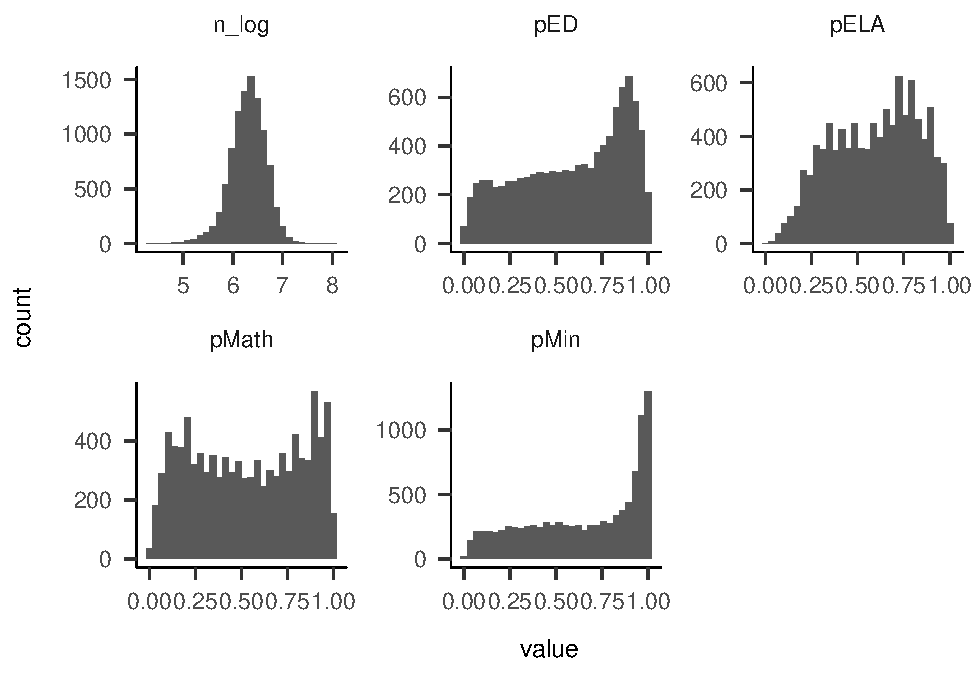
\includegraphics{GenSamp_Paper_files/figure-latex/plot-dist1-1.pdf}
\caption{\label{fig:plot-dist1}Comparison of covariate distributions and their log transformations.}
\end{figure}

\hypertarget{participation-propensity-score}{%
\subsubsection{Participation Propensity Score}\label{participation-propensity-score}}

A response generating model (RGM) was developed to simulate self selection. The RGM creates a propensity score for each school that indicates the probability of the school agreeing to participate if targeted by any of the sampling method. This model assumes that schools can be recruited directly by researchers.

Let and \(\pi^S\) be the participation propensity score. The following base model will be used for the RGM:

\begin{align} \label{eq:sRGM}
  \log\bigg(\frac{\pi^S}{1-\pi^S}\bigg) = \gamma_{0} &+ \gamma_{1}X_{Suburban} + \gamma_{2}X_{Town/Rural} + \gamma_{3}X_{pELL} + \gamma_{4}X_{pED} 
  \\
  &+ \gamma_{5}X_{pMin} + \gamma_{6}X_{MedInc} + \gamma_{7}X_{ELA} + \gamma_{8}X_{Math} \nonumber
\end{align}

where \(X_{Suburban}\) indicates if the school is suburban, \(X_{Town/Rural}\) indicates if the school is in a town or is rural, \(X_{pELL}\) is the percentage of ELL students in the school, \(X_{pED}\) is the percentage of ED students in the school, \(X_{pMin}\) is the percentage of minority students in the school, and \(X_{MedInc}\) is the average median household income in the school community, \(X_{ELA}\) is the percentage of students in a school scoring at or above proficiency on English language arts exams, and \(X_{Math}\) is the percentage of students in a school scoring at or above proficiency on math exams.

To select parameters for the RGM we first identified desireable sample characteristics. Fellers (2017) compared 571 elementary schools that participated in IES funded studies to the full population of U.S. elementary schools on a set of similar covariates, and reported the absolute SMD between the schools that participated and the population. These values served as our \enquote{goal} SMDs (\(SMD^G\)). Iterating across parameter values, we generated \(\pi^S\) and computed the expected mean (\(m^E\)) from a random sample as
\begin{align}
  m^E = \frac{\sum{(\frac{1}{\pi^S} X})}{\sum{\frac{1}{\pi^S}}}
\end{align}

We then calculated the expected SMD (\(SMD^E\)) between a random sample and the population as

\begin{align}
  SMD^E = \frac{m^E - \mu}{\sigma}
\end{align}

Parameter values were selected that minimized the squared difference between the goal and expected SMDs: \(\Delta SMD^2 = (SMD^E-SMD^G)^2\). School differences were not reported for academic outcomes (ELA, Math) and neighborhood median income. However, anecdotal evidence suggests that schools with higher academic performance are less likely to participate in studies. We therefore selected .25 as the goal SMDs for ELA and Math. Indicators of low SES have been shown to be predictive at the district level (Stuart et al., 2017; Tipton et al., 2016) though percentage of students receiving free/reduced lunch were shown to not be predictive of school participation (Fellers, 2017). We therefore also set .25 as the goal SMD for median income.

In conjunction with iterating across parameter values, intercept values were manipulated to generate different levels of population participation rates. Since these rates are unknown, we selected parameters for 9 levels of participation rates. \ref{fig:fig-SMD-goal} reports the difference between our generated SMDs and the goal SMDs for each covariate and each participation rate. \ref{fig:fig-RGM-Pars} reports the parameter values we ultimately selected for each covaraite and each participation rate.

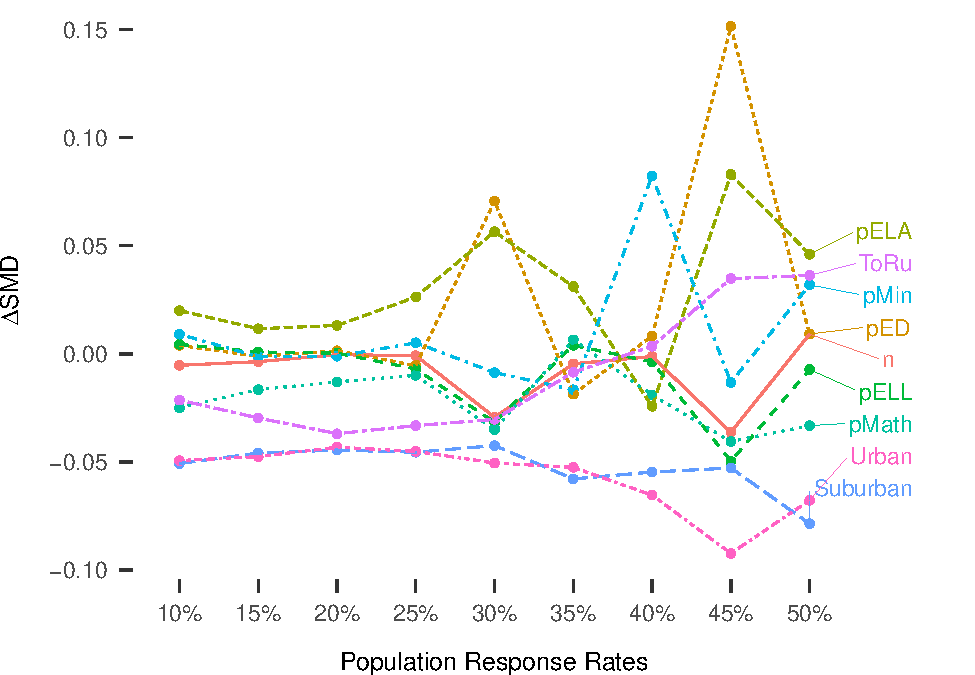
\includegraphics{GenSamp_Paper_files/figure-latex/fig-SMD-goal-1.pdf} 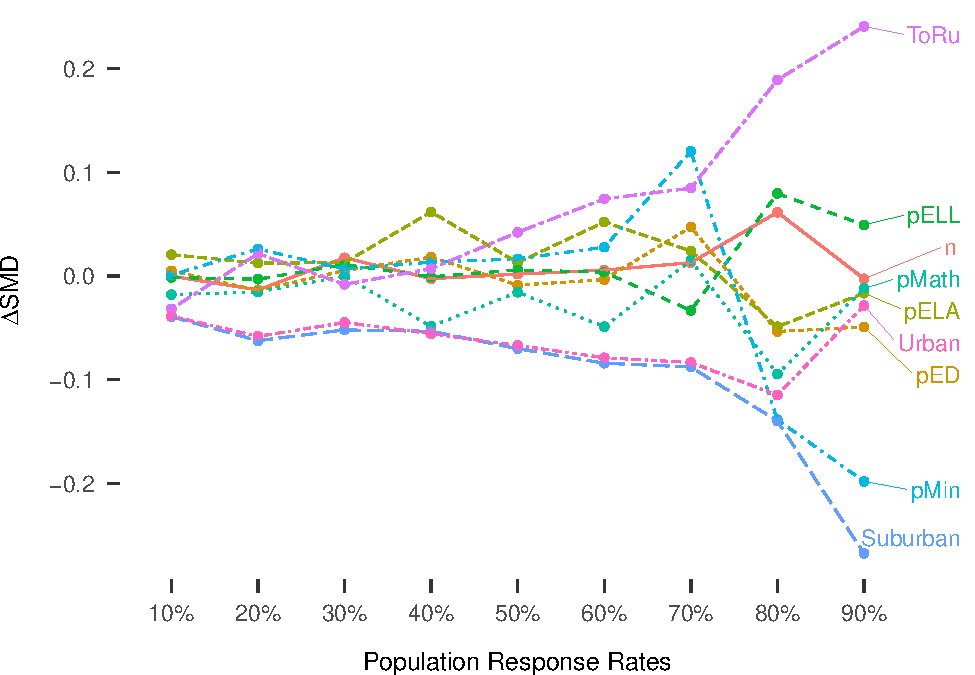
\includegraphics{GenSamp_Paper_files/figure-latex/fig-SMD-goal-2.pdf} 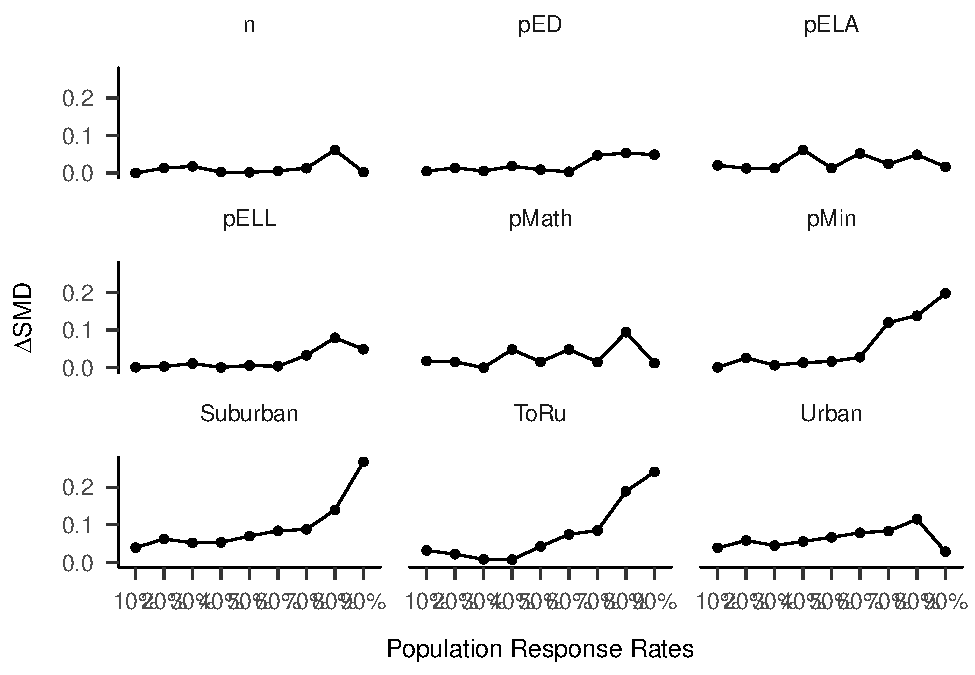
\includegraphics{GenSamp_Paper_files/figure-latex/fig-SMD-goal-3.pdf}

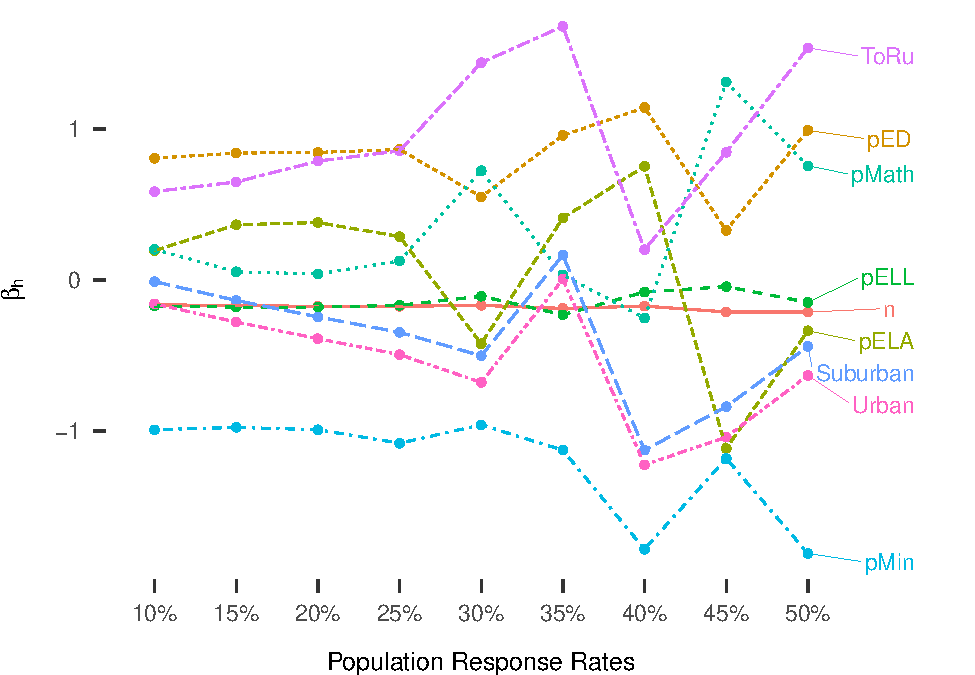
\includegraphics{GenSamp_Paper_files/figure-latex/fig-RGM-Pars-1.pdf} 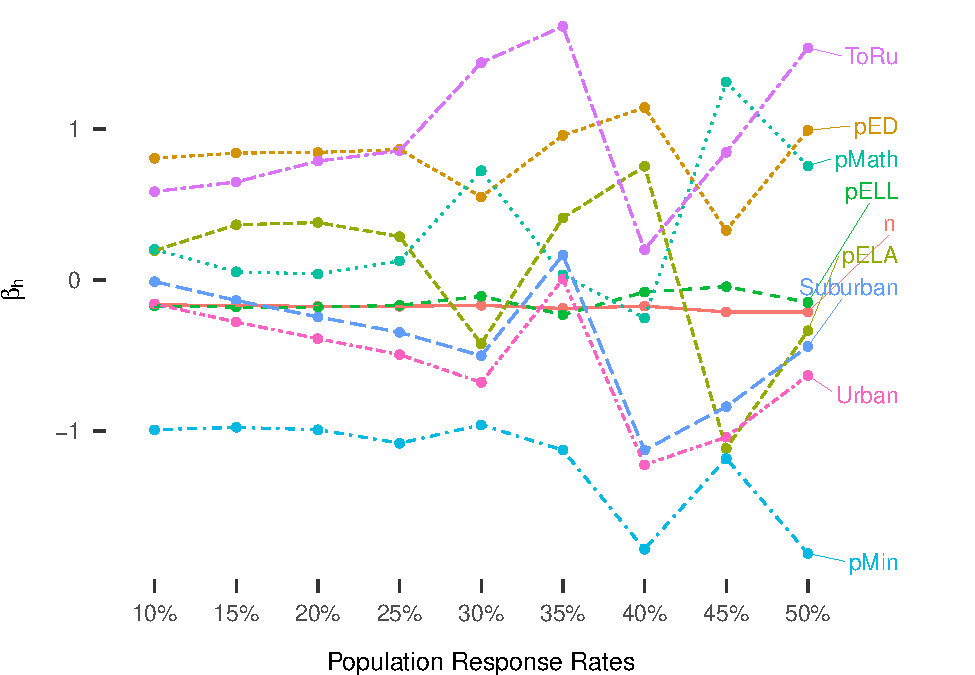
\includegraphics{GenSamp_Paper_files/figure-latex/fig-RGM-Pars-2.pdf}

\hypertarget{stratification}{%
\subsection{Stratification}\label{stratification}}

Stratification was performed prior to simulation because the population is constant across iterations. Per Tipton's (2013) original recommendation, we use k-means clustering to partition the population into strata. This requires selecting a distance metric, choosing the number of strata, and generating the strata.

\hypertarget{number-of-clusters}{%
\subsubsection{Number of Clusters}\label{number-of-clusters}}

Selecting the number of clusters, \(k\), is one of the most difficult problems in cluster analysis (Steinley, 2006). To date, the most extensive investigation of methods for determining \(k\) was conducted by Milligan and Cooper (1985) who analyzed 30 methods. However, aside from the limited generalizability of this study, many methods are also inappropriate in the context of non-hierarchical clustering and thus do not support k-means clustering. Tipton (2013) states that both statistical and practical criteria should be used in selecting the number of clusters. For instance, a large number of clusters would result in more homogeneous strata and, in turn, a more robust sample. However as strata become smaller, they also become more difficult to adequately sample from. Hennig and Liao (2013) argue that the method of selecting \(k\) should depend on the context of the clustering and frame the issue as one of obtaining an appropriate subject-matter-dependent definition of rather than a statistical estimation. Ultimately three considerations were used to select the number of clusters: the ratio of variability between clusters to the sum of within and between cluster variability as recommended by Tipton (2013), a generalized form of the Calinski-Harabasz index (Calinski and Harabasz, 1974) proposed by Hennig and Liao (2013), and the practicality of sampling from fewer clusters.

\begin{figure}
\centering
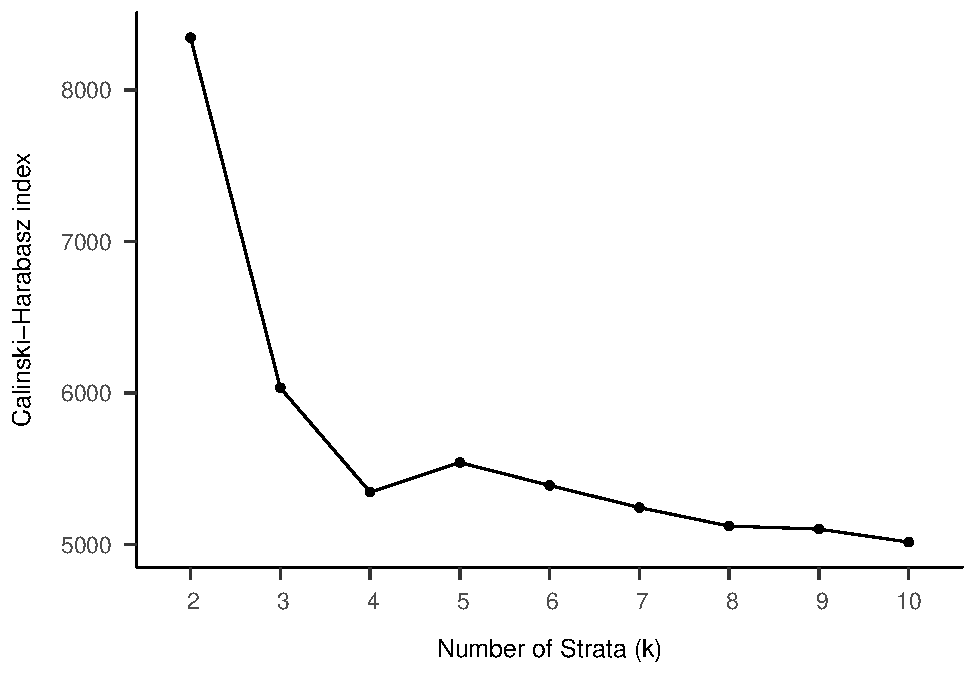
\includegraphics{GenSamp_Paper_files/figure-latex/fig-ch-1.pdf}
\caption{\label{fig:fig-ch}Generalized Calinski-Harabasz index}
\end{figure}

\begin{figure}
\centering
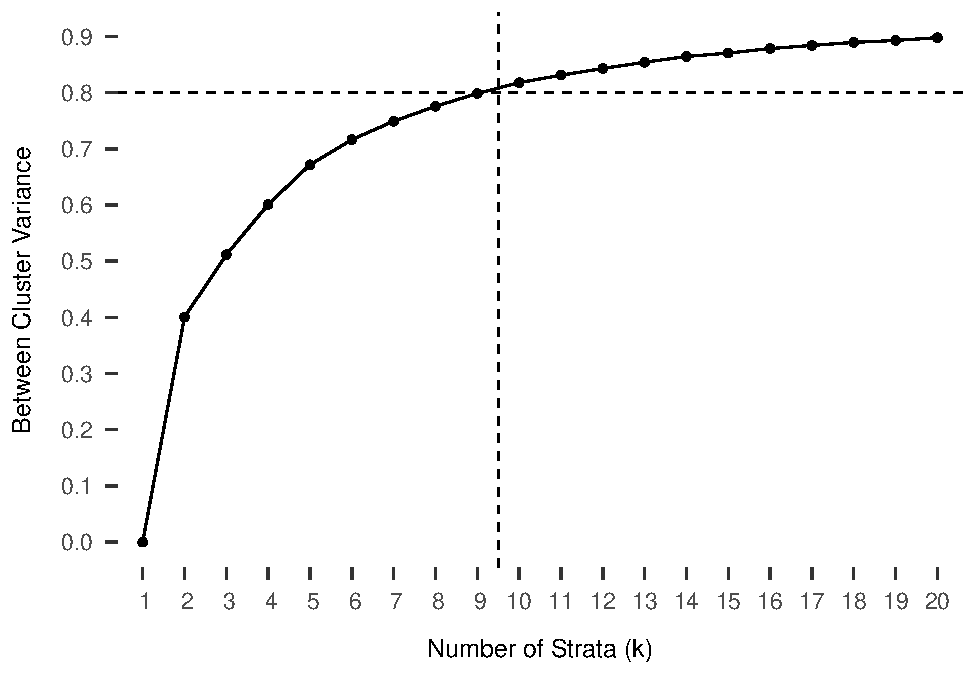
\includegraphics{GenSamp_Paper_files/figure-latex/fig-ratio-1.pdf}
\caption{\label{fig:fig-ratio}Ratio of between cluster sum of squares to total cluster sum of squares}
\end{figure}

\begin{figure}
\centering
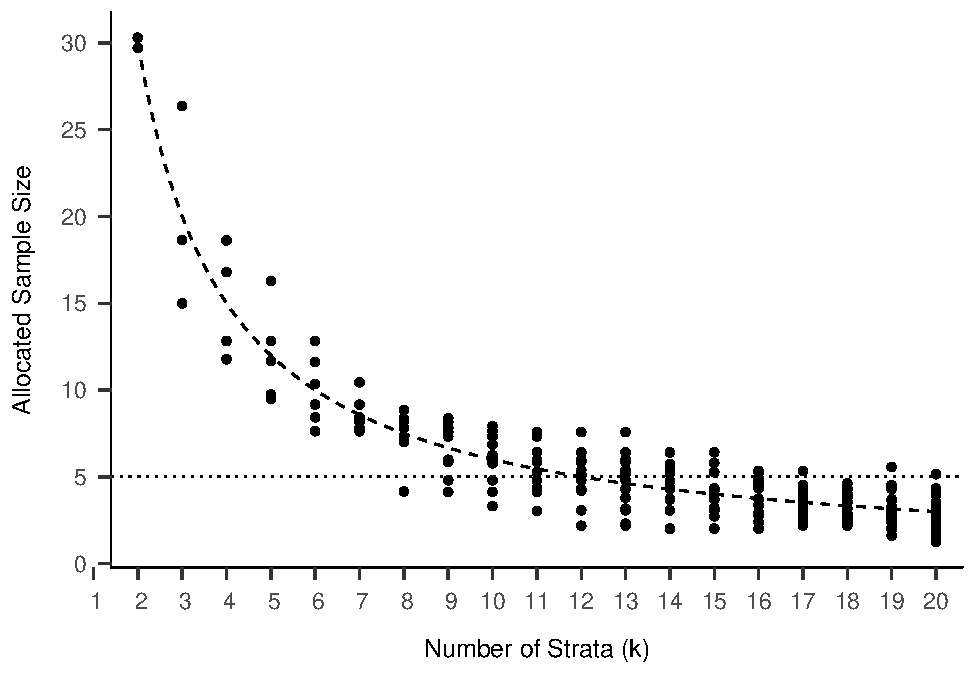
\includegraphics{GenSamp_Paper_files/figure-latex/fig-k-size-1.pdf}
\caption{\label{fig:fig-k-size}Sampling requirements for each cluster}
\end{figure}

\hypertarget{cluster-analysis}{%
\subsubsection{Cluster Analysis}\label{cluster-analysis}}

Cluster analysis was performed using the \emph{cluster} package (Maechler et. al.~2017) in R. First, the \emph{daisy} function is used to compute an \(n\) by \(n\) pairwise distance matrix across all observations. This function requires two parameters: (1) the data matrix, and (2) the distance metric. The data matrix included the full set of school level covariates. The metric was set to \enquote{gower}. Next the \emph{kmeans} function was used to generate clusters. This method uses an optimization algorithm to classify sites into \(k\) clusters by minimizing the total within cluster sum of squares. This function also requires two parameters: (1) the distance matrix, and (2) the number of clusters to generate (\(k\)). For each \(k\), it is recommended to run \emph{kmeans} at least 10 times, and select the clustering that results in the smallest total within-cluster sum of squares. {[}Get Citation{]}

Several methods were used to determine \(k\). Figure \ref{fig:fig-ch} displays the Calinski-Harabasz (CH) index for each \(k\) clusters generated. The value of \(k\) that maximizes the CH index should be selected. However we see several local maxima: \(k = [2, 6, 10, 13]\). Figure \ref{fig:fig-ratio} displays the ration of between-cluster SS to within-cluster SS and plots it against \(k\). Tipton (2013) recommends selecting the number of clusters such that at least 80\% of the variability is between clusters, indicated by the figure as a dashed line. Given this criteria it seems that at least 10 clusters should be generated. However we also see that after a sharp initial increase, the slope of the graph begins to level out. This indicates that as we increase the number of clusters, the benefit of doing so decreases, while the difficulty of sampling from each cluster increases. In that case after 6 or 7 clusters the difficulty of sampling may not be worth such small increases in homogeneity within clusters.

Figure \ref{fig:fig-k-size} plots the sample size that needs to be selected from each cluster to fulfill the proportional allocation requirement such that the number of sites sampled from each cluster is proportional to the size of the cluster in the population. The dashed line indicates the ideal allocation if all clusters were of equal size. We see that when 8 or less clusters are generated, they are more equally sized, with the exception of 3 and 6 clusters where one is much larger than the others. A sensible cutoff may be determined by looking at the size of the smallest cluster. At \(k > 7\) it seems that the smallest clusters would require less than 5 sites being sampled, which may be very difficult in a practical setting. Ultimately 6 clusters were genereated.

\hypertarget{sampling-methods}{%
\subsection{Sampling Methods}\label{sampling-methods}}

Five sampling methods were compared: stratified and unstratified random sampling (SRS, URS), stratified and unstratified convenience sampling (SCS, UCS), and stratified balanced sampling (SBS). For all five methods, the decision of whether or not a school agrees to participate is the same and was generated at the start of every iteration. Let \(J\) be the total number of schools in the population, and let schools be indexed by \(j = 1, ..., J\). We define \(E_j\) as a binary indicator that school \(j\) will agree to participate if contacted by recruiters, where \(E_j = 1\) if the school agrees, and \(E_j = 0\) if the school refuses. Each school was checked for approval by sampling from a Bernoulli distribution with probability equal to \(\pi^S_j\) for each school \(j\)

\begin{align} \label{eq:Ej}
  E_j \sim B(\pi^D_j)
\end{align}

To select a sample, ranks were generated for each school representing the order in which they are approached for recruitment. Schools were sorted by rank, with the all schools up to and including the 60th school where \(E_j = 1\) were considered \enquote{sampled}. Ranks were determined by the sampling method implemented.

\hypertarget{balanced-sampling}{%
\subsubsection{Balanced Sampling}\label{balanced-sampling}}

SBS is unique in that rankings are directly related to school characteristics and do not change across iterations. Ranks within strata are based on equation \eqref{eq:euclid}, where schools that are closer to the \enquote{center} of the strata are more representative of it. Schools will be ranked within strata such that \(r_k= 1\) for the school that is most representative of strata \(k\). The percent of the total sample recruited from each strata should be proportional to the percentage the population of schools that are in the strata (proportional sample allocation). Therefore, schools will be approached independently within each strata in order of rank until the proportional sample allocation requirements are met:
\begin{align} \label{eq:rankCASS}
  \sum_{r_{k}=1}^{R_k}{Z_{r_k} = [\frac{n_k}{N}60}]
\end{align}
where \(n_k\) is the total number of schools in the strata, \(N\) is the total number of schools in the population, and \(R_k\) is the total number of schools approached in strata \(k\) with brackets indicating rounding to the nearest whole number. Though extremely unlikely, several schools and/or districts may have the same rank. In such cases, schools with equal rank will be ordered randomly.

\hypertarget{random-sampling}{%
\subsubsection{Random Sampling}\label{random-sampling}}

In URS, a simple random sample was taken of all the schools in the population. In the context of educational MRTs, this sampling method is impractical. Large subsets of schools are likely to be overlooked if samples are too small, while schools that are sampeld would be randomly scattered throughout the state making data collection and treatment implementation logistically difficult. More effective methods would be clustered randomization, stratified random sampling, or some combination of both. However, the goal here is to uses URS as a high standard for comparison purposes. To achieve this, the order in which schools are approached was indexed by rank, \(r\), where \(r = 1\) if a school is approached first. Rank was randomized such that each school has an equal probability of being approached. Once schools are ranked, each school was approached until 60 schools agree to be in the sample:
\begin{align} \label{eq:rankRS}
  \sum_{r=1}^R{Z^S_r} = 60
\end{align}
where \(R\) is the total number of schools approached. This method allowed tracking of the number of schools that declined to participate, \(R - 60\). For SRS, the same procedure was repeated independantly within strata generated by the cluster analysis. Proportional allocation was used to determine the number of schools to select from each strata.

\hypertarget{convenience-sampling}{%
\subsubsection{Convenience Sampling}\label{convenience-sampling}}

In UCS we assume that recruiters have some knowledge of the schools' likelihoods of participating, and prioritize recruitment based on that knowledge in order to minimize effort. To achieve this, schools were selected one at a time, without replacement, and assigned sequential ranks. Schools were selected with a probability equal to \(\frac{\pi^S}{\sum\pi^S}\) such that schools with a higher \(\pi^S\) were more likely to receive a higher rank. Once a school was selected and assigned a rank, the next school was selected with a probability proportional to the weights of the remaining schools. Once all ranks were assigned, schools were again approached until 60 schools agreed to be in the sample:

\begin{align} \label{eq:rankCS}
  \sum_{r^S=1}^R{Z^S_{r^S} = 60}
\end{align}

As with SRS, in SCS this was performed independantly within strata, and proportional allocation was used to set the target strata sample size.

\hypertarget{analysis}{%
\subsection{Analysis}\label{analysis}}

\hypertarget{generalizability}{%
\subsubsection{Generalizability}\label{generalizability}}

There are several methods to determine how generalizable a sample is to a target population. One common method is to compare the sample to the population on a range of covariates by examining SMDs. Let \(X^r_j\) be the full set of covariates identified in Table \ref{tab:desc} indexed by \(j = 1,...,9\) to the order of \(r\) where \(r = 1,..,3\) if \(X_j\) is continuous and \(r = 1\) if \(X_j\) is binary. Let \(\bar{X^r_j}\) and \(M^r_j\) be the mean of covariate \(X^r_j\) in the sample and population respectively. Finally, let \(\sigma^r_j\) be the standard deviation of \(X^r_j\) in the population. We will calculated the \(SMD\) of each covariate as
\begin{align}
  SMD^r_{j} = \frac{\bar{X}^{r}_{j}-M^{r}_{j}}{\sigma_{j}}
\end{align}

This method is limited as it only provides us with a measure of how close the sample means are to the population means. To have true generalizability, sample variance must also be representative of the population variance. Therefore, in addition to SMDs we also estimated the generalizability index (\(B\); Tipton, 2014). The generalizability index is bounded between 0 and 1, with 0 indicating no overlap between the sample and the population, and 1 indicating the sample is representative of the population. First all sites in the population are divided into \(k\) bins. For bins \(j = 1,...,k\), let \(w_{pj} = N_j/N\) be the proportion of the population and \(w_{sj} = n_j/n\) be the proportion of the sample in each bin. We will calculate \(B\) as:
\begin{align}
  B = \sum^k_{j=1}\sqrt{w_{pj}w_{sj}}
\end{align}
Bins must be defined such that \(\sum{w_{pj}} = \sum{w_{sj}} = 1\). Selecting the correct number of bins is important, as too many bins will underestimate the similarity between distributions, and too few will overestimate. Tipton (2014) recommends generating equal bins of size \(h\) calculated as
\begin{align}
  h = 1.06s(N+n)^{-1/5}
\end{align}
where \(s^2\) is the pooled variance across the sample and population:
\begin{align}
  s^2 = \frac{(n - 1)s^2_s + (N + 1)s^2_p}{(N + n - 2)}
\end{align}

\hypertarget{feasibility}{%
\subsubsection{Feasibility}\label{feasibility}}

In order to assess feasibility, the total number of schools approached to achieve a full sample was tracked. The average number of refusals each sample method resulted in prior to selecting the full sample was calculated across replications. Recruiters expend a lot of resources contacting districts and schools, scheduling meetings and traveling between interested locations. A project with limited resources may not be able to afford to go through a large list of potentially uninterested sites. This measure allows us to compare the difficulty with which a full sample is recruited using each method.

\hypertarget{results}{%
\section{Results}\label{results}}

\hypertarget{generalizability-1}{%
\subsection{Generalizability}\label{generalizability-1}}

Figure \ref{fig:fig-SMD-by-Var} displays the average SMD between the samples and the population for each covariate and at each population participation rate resulting from each sampling method. The dotted horizontal line indicates a cutoff of .25, where SMDs above that indicate large differences between the sample and population for that covariate. Stratified methods consistently performed better than unstratified methods. SBS generally performed as well as or better than SRS. URS often resulted in highly unrepresenative samples except in cases where population participation rates were extremely high.

Figure \ref{fig:fig-avg-Bindex} displays the average \(B\)-index for each method across participation rates. At population participation rates of 60\% and higher, all methods resulted in similarly generalizable samples. However, at lower rates only SBS and SRS consistantly generated highly generalizable samples. SCS and URS performed equally, while UCS resulted in relatively less generalizable samples.

\begin{sidewaysfigure}
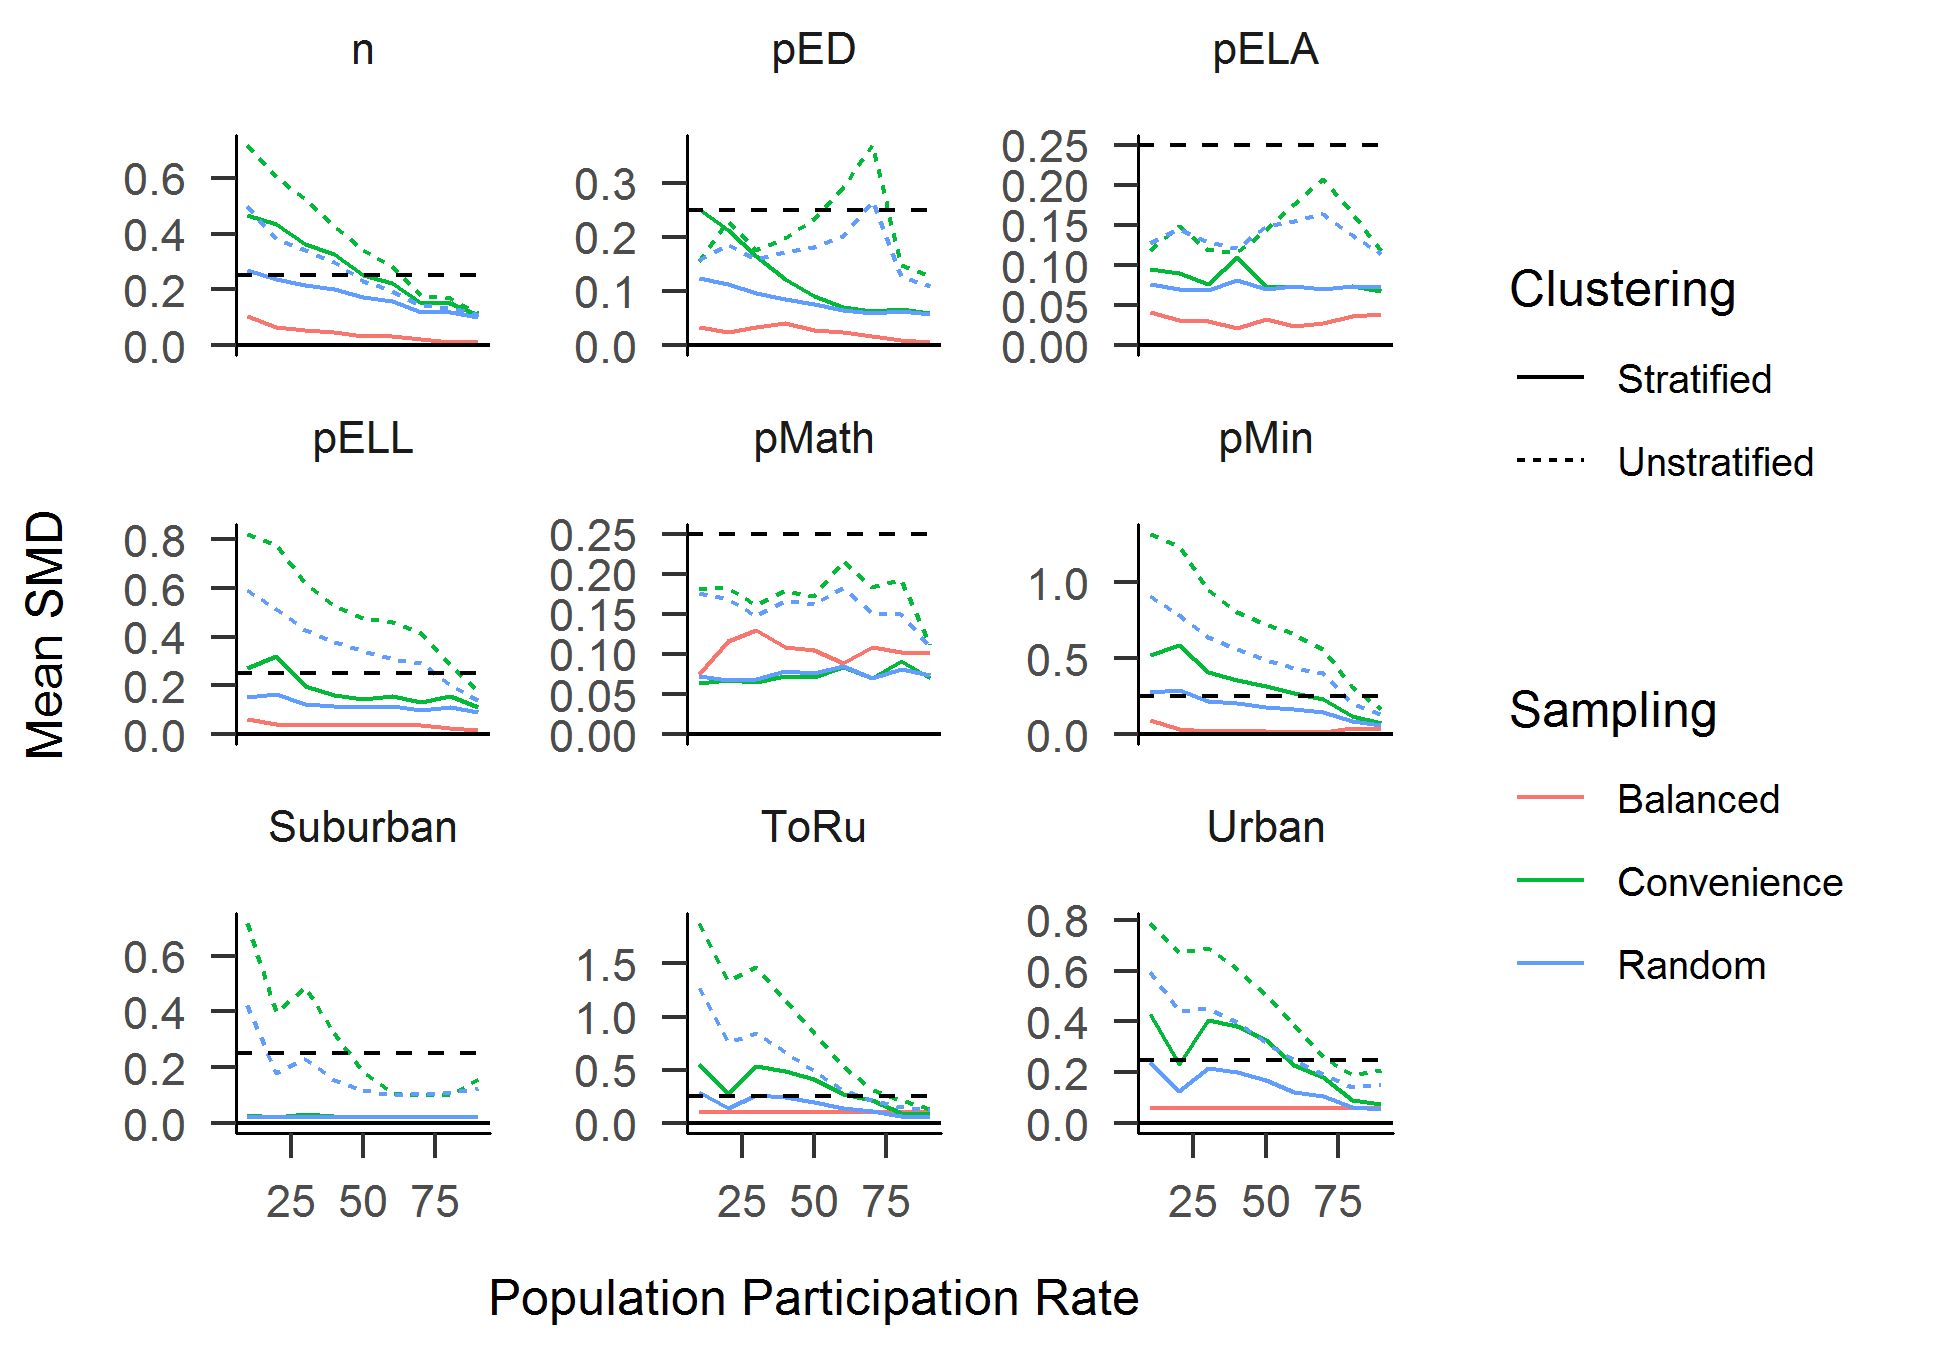
\includegraphics{GenSamp_Paper_files/figure-latex/fig-SMD-by-Var-1} \caption{Averge Standardized Mean Differences between sample and population}\label{fig:fig-SMD-by-Var}
\end{sidewaysfigure}

\begin{verbatim}
## Warning: Detecting old grouped_df format, replacing `vars` attribute by
## `groups`
\end{verbatim}

\begin{figure}
\centering
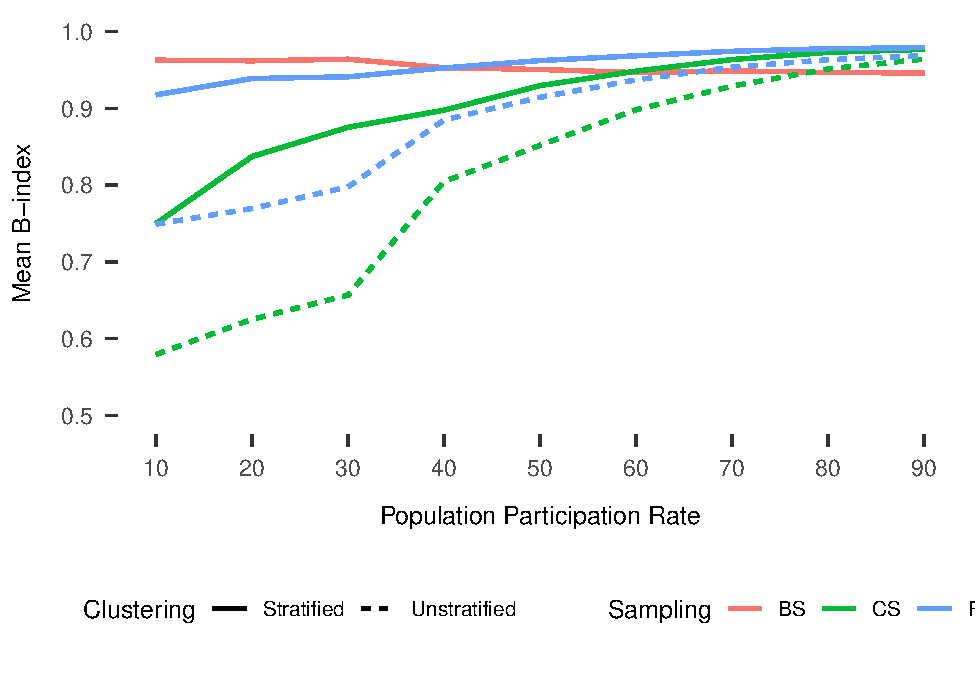
\includegraphics{GenSamp_Paper_files/figure-latex/fig-avg-Bindex-1.pdf}
\caption{\label{fig:fig-avg-Bindex}Averge \(B\)-index for varying participation rates, by sampling method}
\end{figure}

\hypertarget{feasibility-1}{%
\subsection{Feasibility}\label{feasibility-1}}

Figure \ref{fig:fig-units-contacted} reports the average number of schools that needed to be contacted before a full sample of \(N = 60\) schools was selected. At higher participation rates differences between methods were negligibile. However, as participation rates decreased the disparity between the methods became more apparent. Overall, UCS required the least \enquote{effort} to recruit a full sample, followed by URS and SCS, SRS, and finally SBS. Figure \ref{fig:fig-response-rates} plots the participation rates of schools approached for recruitment against the population participation rates. As expected, URS participation rates reflected those in the population. Both UCS and SCS resulted in higher participation rates, while SRS and SBS resulted in lower participation rates.

\begin{verbatim}
## Warning: Detecting old grouped_df format, replacing `vars` attribute by
## `groups`
\end{verbatim}

\begin{figure}
\centering
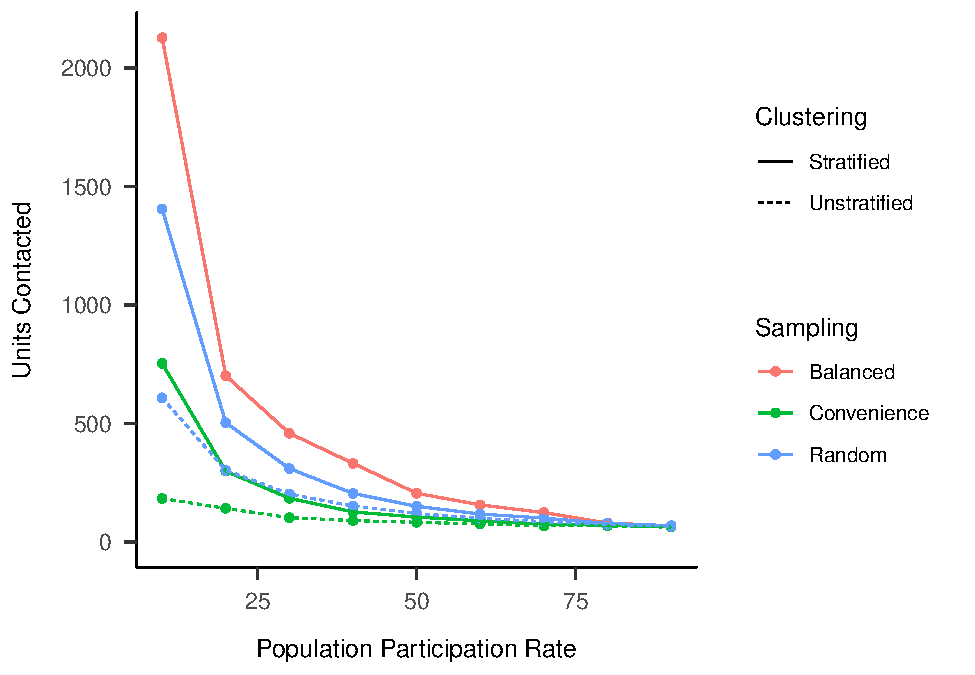
\includegraphics{GenSamp_Paper_files/figure-latex/fig-units-contacted-1.pdf}
\caption{\label{fig:fig-units-contacted}Averge number of schools contacted to achieve N = 60}
\end{figure}

\begin{figure}
\centering
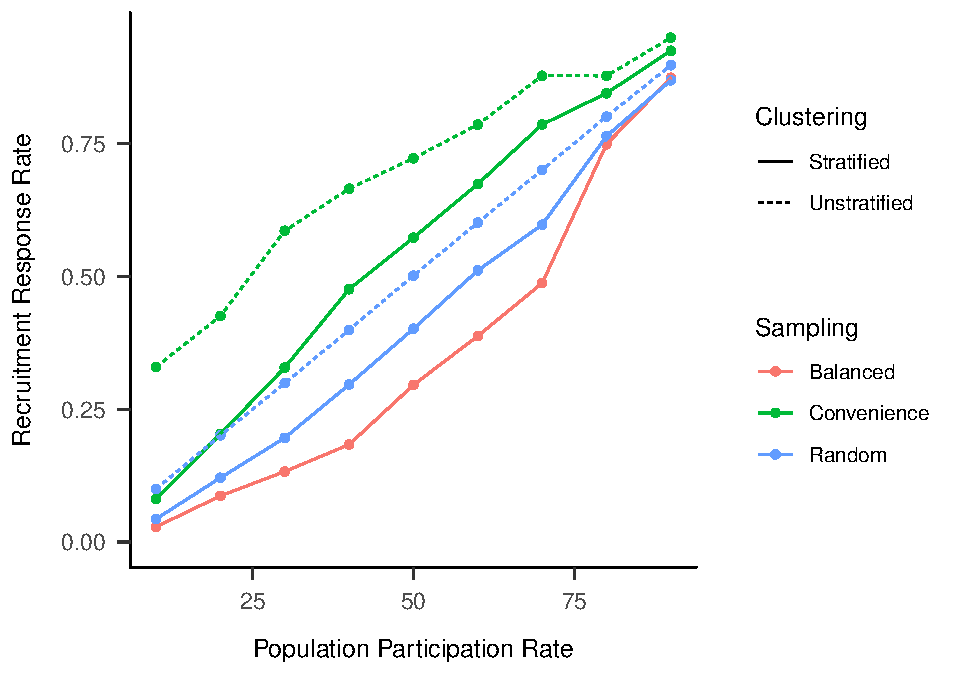
\includegraphics{GenSamp_Paper_files/figure-latex/fig-response-rates-1.pdf}
\caption{\label{fig:fig-response-rates}Recruitment response rates for each sampling method}
\end{figure}

\newpage

\hypertarget{discussion}{%
\section{Discussion}\label{discussion}}

The main goal of this study was to lay a groundwork for exploring the effectiveness and feasibility of sampling methods in the educational context. Our work uncovered several limitations in designing sampling and participation models. The sampling methods we developed made several assumptions about researcher and recruiter behavior in selecting a sample. First, that recruiters always prioritize schools that are most likely to participate. In truth, many other factors play a role such as proximity of sample sites to the researcher and to each other, existing relationships between the recruiters and the sample sites, and other researcher assumptions about the sample site's characteristics. Second, that recruiters have approximiate knowledge of how likely a sampled site is to participate. Though researchers may speculate about sites that are more willing to participate (schools in larger urban distrits) and prioritize recruiting such sites, it is not likely that they would estimate willingness as well as we have simulated. Given this, it is possible that the \enquote{feasibility} of the convenience methods is overestimated.

That said, our participation model is also likely innacurate. The parameters in our response generating model are based on values from a study that examined the difference between schools participating in large-scale randomized control trials (RCT) and the overall population of schools. However, these RCTs themselves typically rely on some form of convenience sampling. In that sense our parameters reflect participation rates of schools that are likely to participate in RCTs, rather than the full population of schools. Furthermore, the decision of whether a school participates in such a study is multi-leveled. Generally, districts serve as gatekeepers, requiring research requests to be submitted and approved before recruitment can begin. If the request is denied, no schools within that district may be recruited. If approved, schools may be contacted individually. The ultimate decision may then rest with administrators, or they may be passed on to teachers most affected by the study.

Despite these limitations, we believe that our findings reasonably represent the relative performance of the various sampling methods we tested in the context of educational research. In terms of selecting a generalizable sample, SBS results in a considerable improvement compared to UCS. However, given the difficulty with which those samples are recruited, SBS is unlikely to be fully implemented in the ideal form. Instead, SCS may be a reasonable compromise. Our findings indicate that any sampling method is greatly improved by first stratifying the population. We show that performing a convenience sample within strata (SCS) is comparable to simple random sampling (URS) both in terms of generalizability and feasibility. URS is considered the gold standard for generalizabilty, however it is not typically implemented due to it requiring substantial resources and other concerns of practicality. The advantage of SCS here is that it enables researchers to mitigate recruitment costs by targeting schools from the same strata that are in close proximity to each other. Beyond generalizability, stratifying in this manner also offers the additional advantage of transparency by forcing the researcher to make sampling decisions in the study design phase, and to keep track of sampling decisions as recruitment is implemented.

Finally, we hope to make clear the disadvantages of convenience sampling in this context. Large scale MRTs are expensive to implement, however by not investing in robust recruitment strategies researchers severly limit the impact and relevance of of their work. We believe that the increased cost of a sampling method designed for generalizability is greatly outweighed by the benefit of an intervention whose impacts we can estimate more accurately and for a wider population.

\hypertarget{references}{%
\section{References}\label{references}}

\begingroup
\setlength{\parindent}{-0.5in}
\setlength{\leftskip}{0.5in}

\hypertarget{refs}{}
\leavevmode\hypertarget{ref-fellersDevelopingApproachDetermine2017}{}%
Fellers, L. (2017). \emph{Developing an approach to determine generalizability: A review of efficacy and effectiveness trials funded by the Institute of Education Sciences} (Ph.D.). Columbia University, United States -- New York. Retrieved from \url{https://search.proquest.com/docview/1865595768/abstract/40FD82F4A0C24535PQ/1}

\leavevmode\hypertarget{ref-gowerGeneralCoefficientSimilarity1971}{}%
Gower, J. C. (1971). A General Coefficient of Similarity and Some of Its Properties. \emph{Biometrics}, \emph{27}(4), 857--871. doi:\href{https://doi.org/10.2307/2528823}{10.2307/2528823}

\leavevmode\hypertarget{ref-grovesSurveyMethodology2004}{}%
Groves, R. M. (Ed.). (2004). \emph{Survey methodology}. Hoboken, N.J: Wiley-Interscience.

\leavevmode\hypertarget{ref-hennigHowFindAppropriate2013}{}%
Hennig, C., \& Liao, T. F. (2013). How to find an appropriate clustering for mixed-type variables with application to socio-economic stratification: How to Find an Appropriate Clustering. \emph{Journal of the Royal Statistical Society: Series C (Applied Statistics)}, \emph{62}(3), 309--369. doi:\href{https://doi.org/10.1111/j.1467-9876.2012.01066.x}{10.1111/j.1467-9876.2012.01066.x}

\leavevmode\hypertarget{ref-kernAssessingMethodsGeneralizing2016}{}%
Kern, H. L., Stuart, E. A., Hill, J., \& Green, D. P. (2016). Assessing Methods for Generalizing Experimental Impact Estimates to Target Populations. \emph{Journal of Research on Educational Effectiveness}, \emph{9}(1), 103--127. doi:\href{https://doi.org/10.1080/19345747.2015.1060282}{10.1080/19345747.2015.1060282}

\leavevmode\hypertarget{ref-olsenExternalValidityPolicy2013}{}%
Olsen, R. B., Orr, L. L., Bell, S. H., \& Stuart, E. A. (2013). External Validity in Policy Evaluations That Choose Sites Purposively. \emph{Journal of Policy Analysis and Management}, \emph{32}(1), 107--121. doi:\href{https://doi.org/10.1002/pam.21660}{10.1002/pam.21660}

\leavevmode\hypertarget{ref-omuircheartaighGeneralizingUnrepresentativeExperiments2014}{}%
O'Muircheartaigh, C., \& Hedges, L. V. (2014). Generalizing from unrepresentative experiments: A stratified propensity score approach. \emph{Journal of the Royal Statistical Society: Series C (Applied Statistics)}, \emph{63}(2), 195--210. doi:\href{https://doi.org/10.1111/rssc.12037}{10.1111/rssc.12037}

\leavevmode\hypertarget{ref-raudenbushStatisticalPowerOptimal2000}{}%
Raudenbush, S. W., \& Liu, X. (2000). Statistical power and optimal design for multisite randomized trials. \emph{Psychological Methods}, \emph{5}(2), 199--213. doi:\href{https://doi.org/10.1037//1082-989X.5.2.199}{10.1037//1082-989X.5.2.199}

\leavevmode\hypertarget{ref-roschelleIntegrationTechnologyCurriculum2010}{}%
Roschelle, J., Shechtman, N., Tatar, D., Hegedus, S., Hopkins, B., Empson, S., \ldots{} Gallagher, L. P. (2010). Integration of Technology, Curriculum, and Professional Development for Advancing Middle School Mathematics: Three Large-Scale Studies. \emph{American Educational Research Journal}, \emph{47}(4), 833--878.

\leavevmode\hypertarget{ref-shadishExperimentalQuasiexperimentalDesigns2002}{}%
Shadish, W. R., Cook, T. D., \& Campbell, D. T. (2002). \emph{Experimental and quasi-experimental designs for generalized causal inference}. Boston, MA, US: Houghton, Mifflin and Company.

\leavevmode\hypertarget{ref-stuartCharacteristicsSchoolDistricts2017}{}%
Stuart, E. A., Bell, S. H., Ebnesajjad, C., Olsen, R. B., \& Orr, L. L. (2017). Characteristics of School Districts That Participate in Rigorous National Educational Evaluations. \emph{Journal of Research on Educational Effectiveness}, \emph{10}(1), 168--206. doi:\href{https://doi.org/10.1080/19345747.2016.1205160}{10.1080/19345747.2016.1205160}

\leavevmode\hypertarget{ref-stuartUsePropensityScores2011}{}%
Stuart, E. A., Cole, S. R., Bradshaw, C. P., \& Leaf, P. J. (2011). The use of propensity scores to assess the generalizability of results from randomized trials: Use of Propensity Scores to Assess Generalizability. \emph{Journal of the Royal Statistical Society: Series A (Statistics in Society)}, \emph{174}(2), 369--386. doi:\href{https://doi.org/10.1111/j.1467-985X.2010.00673.x}{10.1111/j.1467-985X.2010.00673.x}

\leavevmode\hypertarget{ref-tiptonImprovingGeneralizationsExperiments2013}{}%
Tipton, E. (2013a). Improving Generalizations From Experiments Using Propensity Score Subclassification: Assumptions, Properties, and Contexts. \emph{Journal of Educational and Behavioral Statistics}, \emph{38}(3), 239--266. Retrieved from \url{https://www.jstor.org/stable/41999424}

\leavevmode\hypertarget{ref-tiptonStratifiedSamplingUsing2013}{}%
Tipton, E. (2013b). Stratified Sampling Using Cluster Analysis: A Sample Selection Strategy for Improved Generalizations From Experiments. \emph{Evaluation Review}, \emph{37}(2), 109--139. doi:\href{https://doi.org/10.1177/0193841X13516324}{10.1177/0193841X13516324}

\leavevmode\hypertarget{ref-tiptonHowGeneralizableYour2014}{}%
Tipton, E. (2014). How Generalizable Is Your Experiment? An Index for Comparing Experimental Samples and Populations. \emph{Journal of Educational and Behavioral Statistics}, \emph{39}(6), 478--501.

\leavevmode\hypertarget{ref-tiptonSiteSelectionExperiments2016}{}%
Tipton, E., Fellers, L., Caverly, S., Vaden-Kiernan, M., Borman, G., Sullivan, K., \& de Castilla, V. R. (2016). Site Selection in Experiments: An Assessment of Site Recruitment and Generalizability in Two Scale-up Studies. \emph{Journal of Research on Educational Effectiveness}, \emph{9}(sup1), 209--228. doi:\href{https://doi.org/10.1080/19345747.2015.1105895}{10.1080/19345747.2015.1105895}

\leavevmode\hypertarget{ref-tiptonImplicationsSmallSamples2017}{}%
Tipton, E., Hallberg, K., Hedges, L. V., \& Chan, W. (2017). Implications of Small Samples for Generalization: Adjustments and Rules of Thumb. \emph{Evaluation Review}, \emph{41}(5), 472--505. doi:\href{https://doi.org/10.1177/0193841X16655665}{10.1177/0193841X16655665}

\endgroup


\end{document}
